\documentclass[a4paper, 12pt]{article}
\usepackage[utf8]{inputenc}
\usepackage[english,russian]{babel}
\usepackage[T1, T2A]{fontenc}
\usepackage{graphicx}

\usepackage{pgfplots}
\usetikzlibrary{pgfplots.polar}
\pgfplotsset{compat=1.13, grid=major}
\usepackage[left = 2cm, right = 2cm, bottom = 2cm, top = 2cm]{geometry}
\usepackage[top=2cm, left=2cm, right=2cm, left=2cm]{geometry}
\usepackage{amsmath}

\usepackage{tabu}
\usepackage{threeparttablex} 
\usepackage{booktabs} 
\usepackage[tableposition=top]{caption}

\usepackage{subcaption}
\DeclareCaptionLabelFormat{gostfigure}{Рисунок #2}
\DeclareCaptionLabelFormat{gosttable}{Таблица #2}
\DeclareCaptionLabelSeparator{gost}{~---~}
\captionsetup{labelsep=gost}
\captionsetup[figure]{labelformat=gostfigure}
\captionsetup[table]{labelformat=gosttable}
\renewcommand{\thesubfigure}{\asbuk{subfigure}}
\captionsetup[table]{labelformat=simple, labelsep = endash, justification = raggedright, singlelinecheck = off}
\usepackage{indentfirst}
\graphicspath{{image/}}
\newcommand\tline[2]{$\underset{\text{#1}}{\text{\underline{\hspace{#2}}}}$}

% PGFPlots Table ========================================================
\usepackage{pgfplotstable}
\renewcommand{\arraystretch}{1.5}
% recommended:
\usepackage{booktabs}
\usepackage{colortbl}
% pgfplotstable settings
\pgfplotstableset{
	columns/w/.style = {column name = {\boldmath$\omega$}, column type = |c},
	columns/logW/.style = {column name = {\boldmath$\lg{\omega}$}, column type = |c},
	columns/A/.style = {column name = {\boldmath$A(\omega)$}, column type = |c},
	columns/logA/.style = {column name = {\boldmath$20\lg{A(\omega)}$}, column type = |c},
	columns/psi/.style = {column name = {\boldmath$\psi$}, column type = |c|},
	every head row/.style = {before row = \hline},
	after row = {[1mm] \hline},
}

\usepackage{amsmath}
\usepackage{float}

% Table and figure setting ==============================================
\usepackage{threeparttable}
%Change label separator
\usepackage{caption}
\captionsetup[table]{labelformat=simple, labelsep = endash, justification = raggedright, singlelinecheck = off, width = 0.69\textwidth}
\captionsetup[figure]{labelformat=simple, labelsep = endash, name = Рисунок}

% Paragraph indent
\usepackage{indentfirst}
\setlength{\parindent}{15mm}




\begin{document}
	\parindent=1.27cm
	\begin{titlepage}
		\centering
		{\fontsize{12pt}{5cm}\selectfont \bfseries Министерство образования и науки Российской Федерации} \\ \vspace{0.5cm}
		{\fontsize{7pt}{5cm}\selectfont ФЕДЕРАЛЬНОЕ ГОСУДАРСТВЕННОЕ АВТОНОМНОЕ ОБРАЗОВАТЕЛЬНОЕ УЧРЕЖДЕНИЕ ВЫСШЕГО ПРОФЕССИОНАЛЬНОГО ОБРАЗОВАНИЯ} \\ 
		\vspace{1cm}
		{\fontsize{12pt}{5cm}\selectfont \bfseries САНКТ-ПЕТЕРБУРГСКИЙ УНИВЕРСИТЕТ ИНФОРМАЦИОННЫХ ТЕХНОЛОГИЙ, МЕХАНИКИ И ОПТИКИ} \\ \vspace{1.5cm}
		
		{\fontsize{14pt}{5cm}\selectfont Кафедра \hspace{1cm} \underline{Систем Управления и Информатики}  \hspace{1cm} Группа \underline{Р3340}} \\ 
		\vspace{2cm}
		
		{\fontsize{20pt}{5cm}\selectfont \bfseries Лабораторная работа №11} \\
		{\fontsize{20pt}{5cm}\selectfont \bfseries “ИССЛЕДОВАНИЕ МАТЕМАТИЧЕСКОЙ МОДЕЛИ
			ПЬЕЗОЭЛЕКТРИЧЕСКОГО ИСПОЛНИТЕЛЬНОГО
			УСТРОЙСТВА 
			”} \\
		{\fontsize{14pt}{5cm}\selectfont Вариант - 11} \\
		\vspace{1.5cm}
		
		\flushleft
		
		{Выполнил \hspace{2cm} \tline{(фамилия, и.о.)}{9cm} (подпись)} \\
		\vspace{2cm}
		
		{Проверил \hspace{2cm} \tline{(фамилия, и.о.)}{9cm} (подпись)} \\
		\vspace{5cm}
		
		"\underline{\hspace{0.7cm}}"\hspace{0.2cm}\underline{\hspace{2cm}}\hspace{0.2cm}20\underline{\hspace{0.7cm}}г. \hspace{2cm} Санкт-Петербург, \hspace{2cm} 20\underline{\hspace{0.7cm}}г. \\ \vspace{1cm}
		
		Работа выполнена с оценкой \hspace{1cm} \underline{\hspace{8cm}} \\ 
		\vspace{1cm}
		Дата защиты "\underline{\hspace{0.7cm}}"\hspace{0.2cm}\underline{\hspace{2cm}}\hspace{0.2cm}20\underline{\hspace{0.7cm}}г.
		
	\end{titlepage}

\begin{center}
\section*{Задание}
\end{center} \par
\textbf{Целью работы} является изучение математических моделей и исследование характеристик исполнительного устройства, построенного на основе пьезоэлектрического двигателя (ПД) микроперемещений. \par
Необходимо построить схему ПД, которая изображена на рисунке 1 и провести математическое моделирование при различных значениях параметров системы.
\begin{figure}[h!]
\centering
\begin{tikzpicture}
    \draw[thick,->] (0, 3) -- (1, 3) node[anchor = south east] {U};
    \draw[thick] (1, 2.4) -- (1, 3.6) -- (3, 3.6) -- (3, 2.4) -- (1, 2.4);
    \draw (2, 3) node {$\displaystyle{\frac{K_u}{T_us + 1}}$};
    \draw[fill] (3.5, 3) circle (.07); % block with Ku -1
    \draw[thick, ->] (3.5, 3) -- (3.5, 4);
    \draw[thick] (3, 4) -- (4, 4) -- (4, 5) -- (3, 5) -- (3, 4);
    \draw (3.5, 4.5) node {$K_{u}^{-1}$};
    \draw[thick, ->] (3.5, 5) -- (3.5, 5.5) node[anchor = west] {$\hat{U}_p$};
    \draw[thick,->] (3, 3) -- (4, 3);
    \draw[thick] (4, 2.5) -- (4, 3.5) -- (5, 3.5) -- (5, 2.5) -- (4, 2.5);
    \draw (4.5, 3) node {$K_0$};
    \draw[thick, ->] (5, 3) -- (5.75, 3);
    \draw[thick] (6, 3) circle (0.25);
    \draw[thick] (5.82, 2.82) -- (6.18, 3.18); \draw[thick] (6.18, 2.82) -- (5.82, 3.18);
    \draw[fill] (6, 3) -- (6.18, 3.18) arc (45:135:0.25) -- (6, 3);
    \draw[fill] (6, 3) -- (5.82, 2.82) arc (225:315:0.25) -- (6, 3);
    % F_B
    \draw[thick, ->] (6, 4) -- (6, 3.25) node[anchor = south east] {$F_B$};
    % KF
    \draw[fill] (7, 3) circle (.07); % block with Kf
    \draw[thick, ->] (7, 3) -- (7, 4);
    \draw[thick] (6.5, 4) -- (7.5, 4) -- (7.5, 5) -- (6.5, 5) -- (6.5, 4);
    \draw (7, 4.5) node {$K_F$};
    \draw[thick, ->] (7, 5) -- (7, 5.5) node[anchor = west] {$\hat{F}$};
    \draw[thick, ->] (6.25, 3) -- (7.625, 3);
    % gain
    \draw[thick] (7.625, 2.4) -- (8.375, 2.4) -- (8.375, 3.6) -- (7.625, 3.6) -- (7.625, 2.4);
    \draw (8, 3) node {$\displaystyle\frac{1}{m}$}; 
    \draw[thick, ->] (8.375, 3) -- (9.125, 3);
    % integrator
    \draw[thick] (9.125, 2.4) -- (9.875, 2.4) -- (9.875, 3.6) -- (9.125, 3.6) -- (9.125, 2.4);
    \draw (9.5, 3) node {$\displaystyle\frac{1}{s}$}; 
    % Kv
    \draw[fill] (10.25, 3) circle (.07);
    \draw[thick, ->] (10.25, 3) -- (10.25, 4);
    \draw[thick] (9.75, 4) -- (10.75, 4) -- (10.75, 5) -- (9.75, 5) -- (9.75, 4);
    \draw (10.25, 4.5) node {$K_v$};
    \draw[thick, ->] (10.25, 5) -- (10.25, 5.5) node[anchor = west] {$\hat{V}$};
    \draw[thick, ->] (10.25, 3) -- (10.25, 1.5) -- (8.5, 1.5);
    \draw[thick] (8.5, 1) -- (8.5, 2) -- (7.5, 2) -- (7.5, 1) -- (8.5, 1);
    \draw (8, 1.5) node {$K_d$};
    \draw[thick, ->] (7.5, 1.5) -- (6.25, 1.5);
    \draw[thick, ->] (9.875, 3) -- (10.625, 3);
    % integrator
    \draw[thick] (10.625, 2.4) -- (11.375, 2.4) -- (11.375, 3.6) -- (10.625, 3.6) -- (10.625, 2.4);
    \draw (11, 3) node {$\displaystyle\frac{1}{s}$};
    % Kx
    \draw[fill] (12, 3) circle (.07); % block with Kx
    \draw[thick, ->] (12, 3) -- (12, 4);
    \draw[thick] (11.5, 4) -- (12.5, 4) -- (12.5, 5) -- (11.5, 5) -- (11.5, 4);
    \draw (12, 4.5) node {$K_x$};
    \draw[thick, ->] (12, 5) -- (12, 5.5) node[anchor = west] {$\hat{X}$}; 
    \draw[thick, ->] (12, 3) -- (12, 0) -- (8.5, 0);
    \draw[thick] (8.5, -0.5) -- (8.5, 0.5) -- (7.5, 0.5) -- (7.5, -0.5) -- (8.5, -0.5);
    \draw (8, 0) node {$C_p$};
    \draw[thick, ->] (7.5, 0) -- (6, 0) -- (6, 1.25);
    \draw[thick] (6, 1.5) circle (0.25);
    \draw[thick] (5.82, 1.32) -- (6.18, 1.68); \draw[thick] (6.18, 1.32) -- (5.82, 1.68);
    \draw[thick, ->] (6, 1.75) -- (6, 2.75);
    \draw[thick, ->] (11.375, 3) -- (13, 3) node[anchor = south east] {$x$};
\end{tikzpicture}
\caption{Структурная схема пьезоэлектрического исполнительного устройства}
\end{figure} \par
Параметры данной схемы указаны в таблице 1.

\begin{table}[h!]
    \centering
    \begin{threeparttable}
        \caption{параметры пьезоэлектрического двигателя}
        \begin{tabular} {|c|c|c|c|c|c|}
            \hline
            $C_p$ & $m$ & $K_0$ & $K_d$ & $T_u$ & $F_B$ \\
            Н/м & кг & Н/В & Н$\cdot$с/м & мс & Н \\ \hline
            $2 \cdot 10^6$ & 0.125 & 7.5 & $0.9 \cdot 10^2$ & 0.15 & 4 \\ \hline
        \end{tabular}
    \end{threeparttable}
\end{table}
\newpage
\begin{center}
	\section{Анализ пьезоэлектрического двигателя}
\end{center}

\begin{figure}[h]
	\centering
	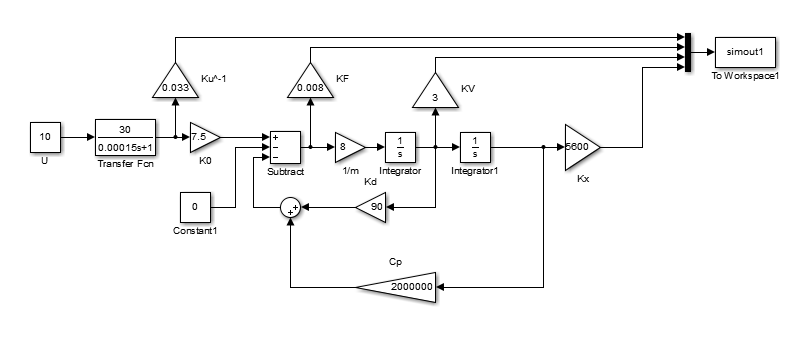
\includegraphics[width=1\linewidth]{0}
	\caption{Схема моделирования}
	\label{fig:0}
\end{figure}
Для соответствия выходного сигнала уровню 10, необходимо его домножить на коэффициент, рассчитанные коэффициенты:\par
$K_{U}^{-1}$=0.033\par
$K_{F}$=0.008\par
$K_{V}$=3\par
$K_{X}$=5600\par
 
\newpage
	\begin{figure}[h]
		\centering
		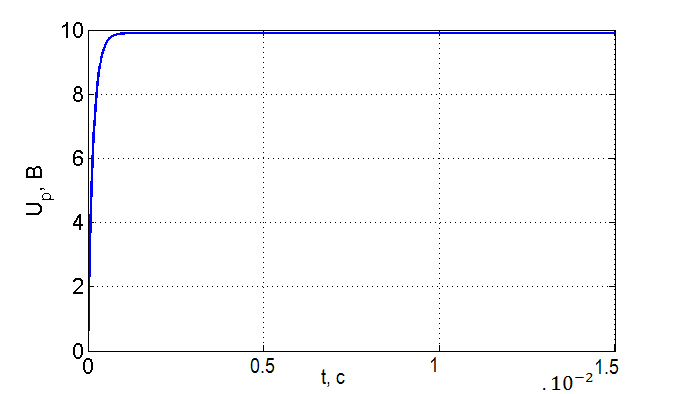
\includegraphics[width=0.85\linewidth]{1}
		\caption{Графика переходного процесса $U_p(t)$}
		\label{fig:1}
	\end{figure}
	\begin{figure}[h]
		\centering
		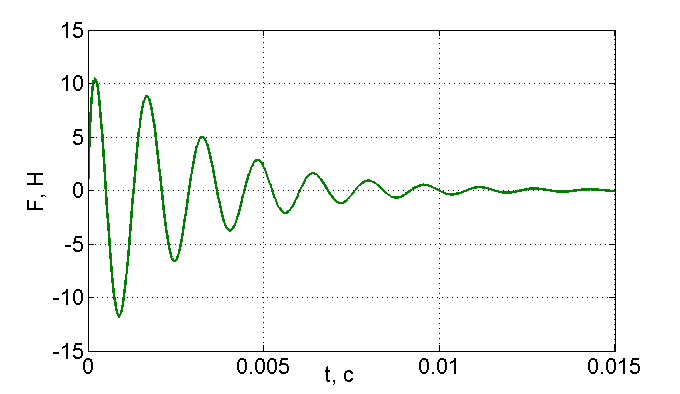
\includegraphics[width=0.85\linewidth]{2}
		\caption{Графика переходного процесса $F(t)$}
		\label{fig:2}
	\end{figure}
\newpage
	\begin{figure}[h]
		\centering
		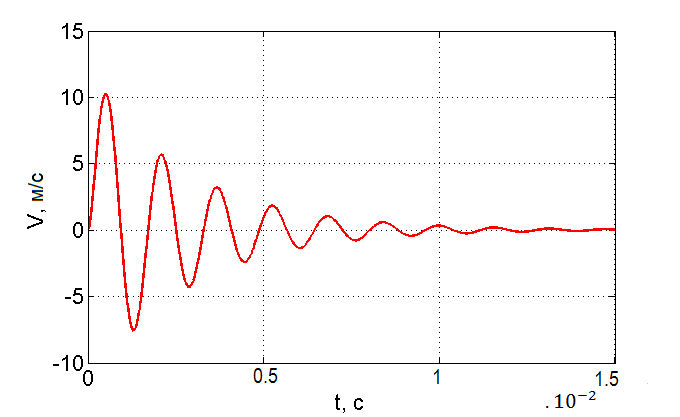
\includegraphics[width=0.8\linewidth]{3}
		\caption{Графика переходного процесса $V(t)$}
		\label{fig:3}
	\end{figure}
	\begin{figure}[h]
		\centering
		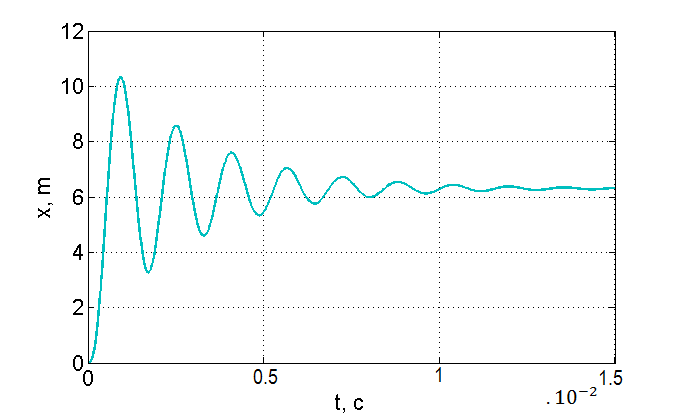
\includegraphics[width=0.8\linewidth]{4}
		\caption{Графика переходного процесса $x(t)$}
		\label{fig:4}
	\end{figure}

\newpage
\begin{center}
	\section{Исследование влияния массы нагрузки m на вид переходных процессов}
\end{center}\par

	\begin{table}[h!]
		\centering
		\begin{threeparttable}
		
	\caption{Характеристики системы при различной массе нагрузки }
	\renewcommand{\arraystretch}{1}
	\renewcommand{\tabcolsep}{0.9cm}
	\begin{tabular}{|c|c|c|c|}
		\hline
		m, кг	&	0.0625	&	0.125	&	0.1875		\\
		\hline
		tп,мс	&	0.259	&	0.326	&	0.379		\\
		\hline
		$\sigma, \%$	&	49	&	63.9	&	70.9		\\
		\hline
		$x,10^{-3}м$	&	0.113	&	0.113	&	0.113		\\
		\hline
	\end{tabular}
\end{threeparttable}
\end{table}

Иземеняя массу нагрузки в пределах $[0.5m, 1.5m]$ получим различные виды переходных процессов с различными значениями преререгулирования $\sigma$, времени переходных процессов $t_\text{п}$, и установившегося значения выходного сигнала $x_\text{уст}$. Полученные значеня представлены в таблице 2.

\begin{figure}[h]
	\centering
	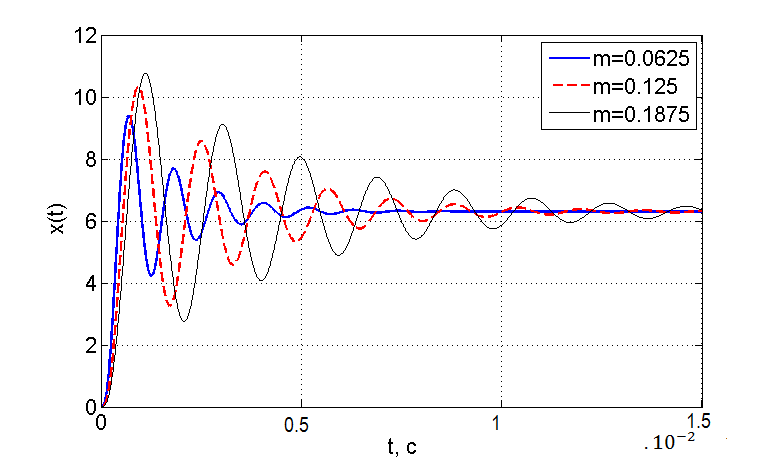
\includegraphics[width=0.9\linewidth]{12}
	\caption{Графика переходного процесса при измении массы}
	\label{fig:5}
\end{figure}
\newpage


\begin{center}
	\section{Исследование влияния постоянной времени на вид переходных процессов}
\end{center}

Передаточная функция системы:\\
\begin{equation}
W(s)=\frac{K_UK_0}{T_Ums^3+(m+K_dT_U)s^2+(K_d+C_pT_U)s+C_p}
\end{equation}\par
В таблице 3 приведена зависимость характеристик системы от постоянной времени и расчитанные корни передаточной функции(1). 
  
\begin{table}[h!]
	\begin{threeparttable}
\caption{Характеристики системы при различной постоянной времени  }
\renewcommand{\arraystretch}{1}
\renewcommand{\tabcolsep}{0.75cm}
\begin{tabular}{|c|c|c|c|c|}
	\hline
	Tu,мс	&	0.15	&	0.3	&	0.6	&	0.9	\\
	\hline
	tп,мс	&	0.326	&	0.393	&	0.536	&	0.773	\\
	\hline
	$\sigma$, \%	&	63.9	&	44.3	&	14.1	&	5.63	\\
	\hline
	$x,10^{-3} \text{ м}$	&	0.113	&	0.113	&	0.113	&	0.113	\\
	\hline
	$s_1, 10^{3}$	&	-6.67	&	-3.33	&	-1.67	&	-1.11	\\
	\hline
	$s_2, 10^{3}$	&	-0.36-3.98i	&	-0.36-3.98i	&	-0.36-3.98i	&	-0.36-3.98i	\\
	\hline
	$s_3, 10^{3}$	&	-0.36+3.98i	&	-0.36+3.98i	&	-0.36+3.98i	&	-0.36+3.98i	\\
	\hline
\end{tabular}
\end{threeparttable}
\end{table}\par

На рисунке 8 приведены графики переходных процессов системы при изменении постоянной времени.
\begin{figure}[h]
	\centering
	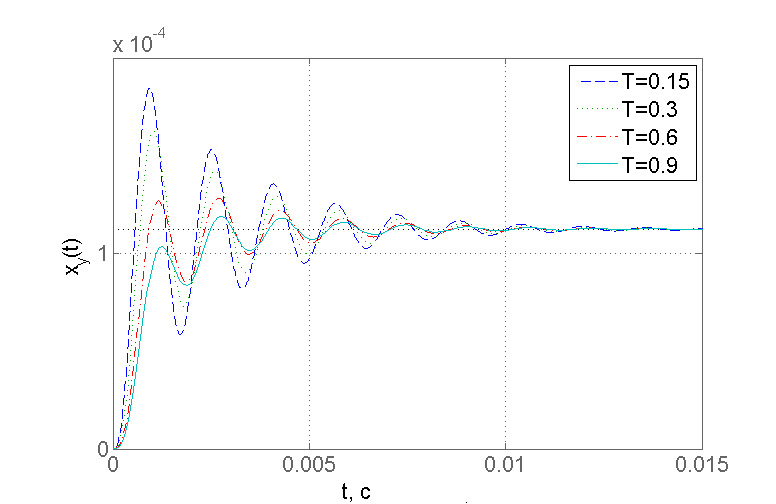
\includegraphics[width=0.9\linewidth]{8}
	\caption{Графика переходного процесса при изменению $T_{\mu}$}
	\label{}
\end{figure}

С увеличением постоянной времени высоковольтного усилителя снижает перерегулирование и время переходного процесса. На установившееся значение перемещения постоянная времени не влияет

\newpage
\begin{center}
	\section{Исследование влияния коэффициента упругости $C_p$}
\end{center} \par
Исследуем поведение системы, варьируя $C_p$, при выключенном питании $U = 0$ и приложенном воздействии $F_B = 4$. На рисунке 9 и 10 представлены полученные в результате математического моделирования переходные процессы при различных $C_p$.

\begin{figure}[h]
	\centering
	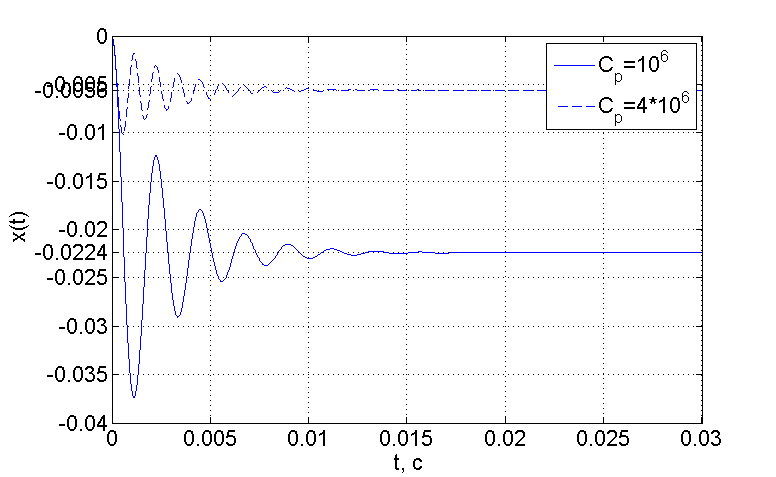
\includegraphics[width=0.9\linewidth]{9}
	\caption{Графика переходного процесса $x(t)$ при изменению $C_{p}$}
	\label{}
\end{figure}
\begin{figure}[h]
	\centering
	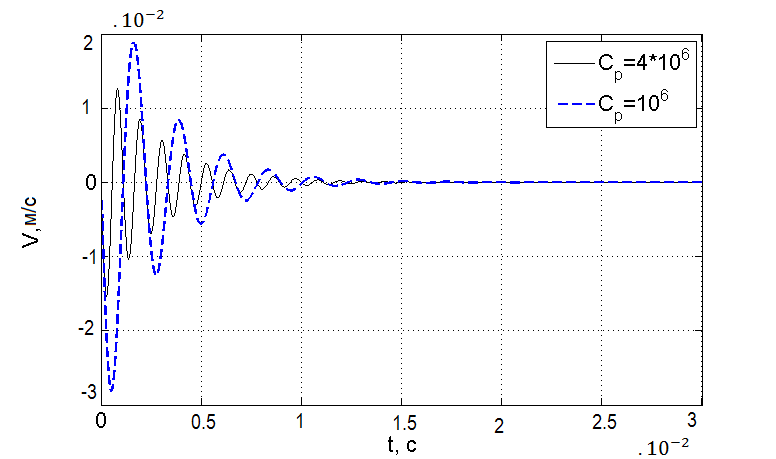
\includegraphics[width=0.9\linewidth]{11}
	\caption{Графика переходного процесса $V(t)$ при изменению $C_{p}$}
	\label{}
\end{figure}
\newpage
Из передаточной функции (1) мы построим ЛАЧХ системы\par 


\begin{equation}
W(s) = \frac{{{K_U}{K_0}}}{{{T_u}m{s^3} + (m + {K_d}{T_u}){s^2} + ({K_d} + {C_p}{T_u})s + {C_p}}}
\end{equation}

\begin{equation}
W(jw) = \frac{{{K_U}{K_0}}}{{({C_p} - m{w^2} - {K_d}{T_u}{w^2}) + j({C_p}{T_u} + {K_d}w - {T_u}m{w^3})}}
\end{equation}

\begin{equation}
A(w) = \frac{{{K_U}{K_0}}}{{\sqrt {{{({C_p} - m{w^2} - {K_d}{T_u}{w^2})}^2} + {{({C_p}{T_u} + {K_d}w - {T_u}m{w^3})}^2}} }}
\end{equation}

\begin{equation}
L(w) = 20\lg A(w)
\end{equation}

\begin{figure}[h]
	\centering
	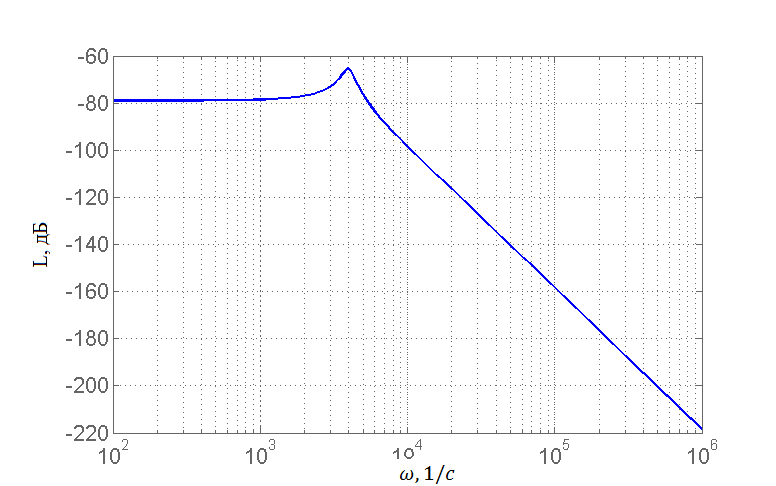
\includegraphics[width=0.7\linewidth]{10}
	\caption{Графика ЛАЧХ системы}
	\label{}
\end{figure}
\newpage
\begin{center}
	\section*{Выводы}
\end{center}\par

В работе была исследована математическая модель и зависимости переходных процессов исполнительного устройства, построенного на основе пьезоэлектрического двигателя микроперемещений, от его параметров и внешних воздействий\par
При увеличении массы нагрузки $m$, увеличивается перерегулирование $\sigma$ и время переходных процессов $t_\text{п}$. \par
При увеличении постоянной времени $T_u$, уменьшается значение перерегулирования, и времени переходного процесса. \par
При увеличи коэффициента упругости $C_p$ уменьшается влияние сил системы и как следствие снижается амплитуда колебания и установившееся значение $x_\text{уст}$.
\end{document}